\documentclass[a4paper]{article}
\usepackage[T1]{fontenc}
\usepackage[utf8]{inputenc}
\usepackage{lmodern}
\usepackage{amsmath,amssymb}
\usepackage[top=3cm,bottom=2cm,left=2cm,right=2cm]{geometry}
\usepackage{fancyhdr}
\usepackage{mathabx}
\usepackage{esvect,esint}
\usepackage{xcolor}
\usepackage{tikz,circuitikz}\usetikzlibrary{calc}
\usepackage{graphicx}
\usepackage{minted}
\title{Systèmes d'exploitation\\Rapport de projet - Réseaux de Kahn}
\author{Sylvain Brisson - Arthur Rousseau}
\date{}
\parskip1em\parindent1pt\let\ds\displaystyle


\begin{document}
\maketitle
\noindent

\section{Implémentations de réseaux de Kahn}

Les réseaux de Kahn (en anglais, KPN: Kahn process networks ) sont un modèle de calcul distribué dans lequel un groupe de processus communiquent entre eux à travers des FIFO. Sous la condition d'être composés de processus déterministes ces réseaux sont déterministes. Ces réseaux trouvent des applications dans la réaslisation de systèmes distribués.

Ce projet à pour but de réaliser différentes implémentations d'une interface de KPN, les implémentations réalisées sont:
\begin{itemize}
    \item Une implémentation basée sur des processus lourds Unix sommuniquant par des pipes
    \item Une implémentation basée sur des processus lourds Unix sommuniquant par des sockets
    \item Une implémentation séquentielle 
    \item Une implémentation basée sur une implémentation MPI en OCaml
    \item Une implémentation en C basée sur des processus Unix communiquant par des pipes
\end{itemize}

\subsection{Version Unix pipes: processus lourds avec communication via pipes}

Code: \verb|Version_Unix.ml|

Cette implémentation repose sur des processus lourds, initiés par des appels fork (fork(2)), et communiquant via des pipes (pipe(2))

L'initiation d'un canal repose sur l'ouverture d'une pipe et la construction de canaux de communications OCaml (\mintinline{OCaml}{in_channel}, \mintinline{OCaml}{out_channel}) à partir les descripteurs de fichiers de l'entrée et de la sortie de la pipe. L'écriture et la lecture sur les canaux se font de manière générique selon les types par marshalling (module \verb|Marshal| OCaml).

\subsection{Version Unix sockets: processus lourds avec communication via sockets}

Code: \verb|Version_Sockets.ml|

Comme la précédente cette implémentation repose elle aussi sur des processus lourds mais communiquant via des sockets.

L'implémentation réalisée ne permet que des communications locales, les ports sont attribués de manière automatique (1 port en local pour chaque canal de communication).

L'initiation d'un canal commence par la construction d'une adresse (INET) locale, l'ouverture de 2 sockets (une pour la partie serveur et une pour la partie client) le lien de la socket serveur à l'adresse (bind(2)) et le démarrage du serveur (listen(2)) puis la connection du client au serveur (connect(2)). Les descripteurs de fichier des sockets sont ensuite convertis en canaux de communication OCaml.

Dans l'état des choses cette implémentation de permet rien de plus que l'implémentation basée sur une communication via pipes.

\subsection{Version séquentielle}

<<<<<<< HEAD
Code: \verb|Version_sequentielle.ml|

Cette implémentation utilise une queue pour stocker les actions à effectuer (notamment pour le \texttt{doco}), avec des fonctions \texttt{add} pour ajouter une action à la queue et \texttt{suivant} pour exécuter la première action de la queue.

La création d'un processus se ramène alors à \texttt{add} et l'exécution à \texttt{suivant}.

Les canaux sont eux aussi des queues. 

\subsection{Version MPI}

Code: \verb|versionMPI.ml|

Cette dernière version repose sur le module MPI de OCaml (https://github.com/xavierleroy/ocamlmpi).

\textbf{Note sur MPI}

MPI (Message Passing Interface) est une norme de bibliothèque permettant la distribution de calculs sur des clusters à mémoire partagée ou non. On utilise ici l'implémentation opensource OpenMPI (utilisable depuis C et fortran) et le module MPI OCaml (basée sur la bibliothèque C). Dans une application MPI tous les processus éxécutent le même code mais avec des valeurs différentes de la variable \verb|rank| (prenant des valeurs de 1 à $N$, $N$ le nombre de processus). Les commnications points à point se font alors en indiquant le rang du processus source/destination et \verb|tag|, un entier. MPI repose sur des processus lourds, elle ne permet pas de lancer plus de processus qu'il n'y à de slots (coeurs de processeurs, x2 si multithreading) pour minimiser les temps de calcul.

\textbf{Utilisation pour implémentation de KPN}


Les canaux de communication sont idenifiés par un entier (\verb|tag|).

L'appel à doco lance le processus $k$ dans le processus $k\mod{N}$.


\subsection{Implémentation en C}

Code: \verb|kahn.c| \verb|kahn.h|

On réalise une implémentation en C d'une bibliothèque de réseaux de Kahn basée sur des processus lourds Unix communiquant via des pipes.

Les canaux de commmunications sont les descripteurs de fichiers renvoyés par les appels pipe, les communication se font par appels write et read, les processus sont représentés là aussi par un couple d'une fonction (pointeur vers une fonction) et des paramètres associés.

Les prototypes des fonctions ne respectent par l'interface fournies en OCaml: les fonctions put et get nécessitent la taille du buffer à envoyer et le type des données.

\subsection{Tests simples des implémentations}

On test les implémentations avec le test fourni: un processus \verb|integer| génère une suite infinie d'entier (dans l'ordre depuis 1) et les envoi à une autre processus \verb|output| qui affiche ce qu'il reçoit sur la sortie standard.

\section{Applications directe des implémentations}
\subsection{Crible}
Le crible présenté est inspiré de celui du TP5. Il fait passer chaque entier par une suite de filtres (\texttt{sift}), où chaque filtre teste la divisibilité par un nombre premier. Si on rencontre un nombre premier, on crée un nouveau filtre.
\subsection{Algorithme de Strassen}
L'algorithme de Strassen implémenté crée un nouveau processus pour chaque multiplication.

\section{Implémentation MPI basée sur les réseaux de Kahn}

\subsection{Implémentation}

A partir de l'implémentation en C de KPN on réalise une implémentation de l'interaface minimale MPI \verb|mpi_subset.h|.

L'utilisation interne de la bibliothèque est identique à l'utilisation de la bibliothèque C standard: appel à MPI\_Init() puis récupération des varibles rank et size (rang du processus et taille du communicateur) puis suite du programme à comportement dépendant de ces deux variables.

Les limites de l'implémentation sont:
\begin{itemize}
    \item Les tag ne sont pas implémentés
    \item Les wildcards pour la réception ne sont pas implémentées
    \item Seules les communications point à point bloquantes sont implémentées
\end{itemize}

La documentation est dans \verb|mpi_subset.h|, les détails de l'implémentation à partir des KPN dans \verb|mpi_subset.c|.

L'utilisation diffère de l'utilisation classique (execution avec mpirun), on lance ici directement l'éxécutable issu de la compilation avec comme option -np (ou -n) pour indiquer le nombre de processus à lancer.

\subsection{Exemples d'utilisation}

On réalise des scripts C utilisant l'implémentation MPI réalisée:
\begin{itemize}
    \item \verb|test_hello.c| : programme minimal MPI, avec synchronisation
    \item \verb|test_pi.c| : programme calculant une valeur approchée de $\pi$ (formule de Madhava-Leibniz)
    \item \verb|FEM_MPI.c| :  programme de résolution de l'équation de d'Alembert en milieu homogène non dispersif non absorbant par méthode des différences finies (FEM). les résultats sont écrits sous format netCDF, pour comparaison sont fournis les programmes \verb|FEM.c| (idem mais non parallélisé), \verb|FEM_MPI_REF.c| (idem mais faisant appel à une implémentation MPI complète, testé avec OpenMPI)
\end{itemize}

\subsection{Résultats}

On réalise un benchmarking trivial pour évaluer les performances de la paralléisation pour les scripts de FEM et de calcul de $\pi$

\begin{itemize}
    \item \verb|test_pi.c| (réalisé avec \verb|benchmark_PI_MPI.bash|)
    \begin{figure}[!ht]
        \centering
        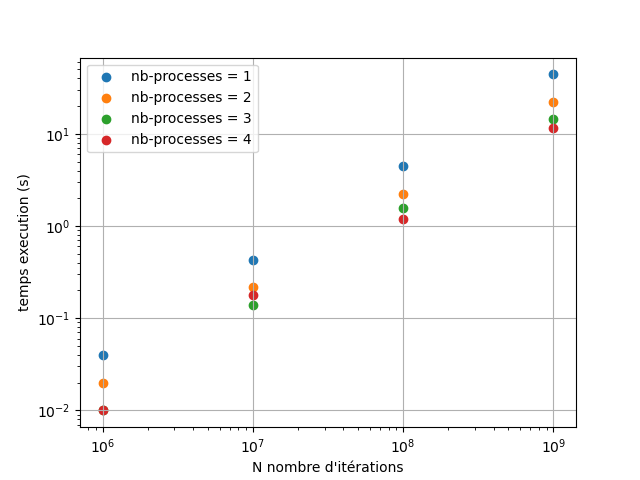
\includegraphics[width=0.5\linewidth]{../MPI_Kahn_C/test/data-benchmark/plot_pi_benchmark.png}
        \caption{Résultats du benchmark}

    \end{figure}
\end{itemize}

Pour des grands nombre d'itération, le temps de calcul suit l'inverse du nombre de processus.



\end{document}